\subsection{Test Configuration}

DEF is designed to be transparently compatible with C in that C header files can be included in DEF, and the utility \texttt{defghi} (DEF Generate Headers and Interfaces), can take DEF source files and emit C header files for inclusion in C.  This makes it easy to correct for any variation created by the benchmark driver or the allocator.

Our benchmark was tested on a 72-core (4 sockets with 18 cores each capable of running 2 hardware threads, totalling 144 hardware threads) Intel Xeon machine clocked at 2.50 GHz with 512 GB of RAM and 4 memory banks. The machine is running Ubuntu 14.04 with kernel verion 3.13.0-141. The with DEF code was compiled with DEF version (Whatever) and the C code was compiled with Clang 6.0, and all code was compiled with -03 level of optimisation.

During the benchmark threads were pinned programmatically to inidvidual cores initially avoiding HyperThreading and later exhausting all inidivual exection units on a single CPU with the use of HyperThreading, before migrating to another CPU socket. The scalable JEMalloc (cite JEMalloc and find version) allocator was used in all tests. The \texttt{numactl} Linux program was used to control which memory bank allocation was allowed to take place. The memory banks closest to the running CPUs were selected as they became active.

The microbenchmark measures the number of operations carried out over a specified amount of time rather than the time taken to exectute a specified number of iterations. The rational for this is threads finish their iterations before other threads. The remaining threads complete their iterations with less contention in the system, skewing the overall benchmark. Our benchmark reports the number of operations per second. The primary comparison is between the leaky C and the forkscan enabled DEF implementations. Each benchmark is run for a total of 20 seconds each, with each configuration being sampled 5 times. The average of the runs is plotted with error bars show the maximum variation in each run.

Initially we present a relative performance graph to demonstrate the relative performance of DEF to C, showing the performance as a percentage. Our results shows that DEF achieves very comparable performance to C in the single threaded leaky benchmark. The other graphs represent a more typical comparison of operations per second in the aggregate of all threads. Two performance loads were tested for the set data-structures of 10 and 20 percent updates (insertion and deletion) respectfully. The priority queue data-structures alternated between inserting a random item and popping the minimum entry.


\begin{figure}
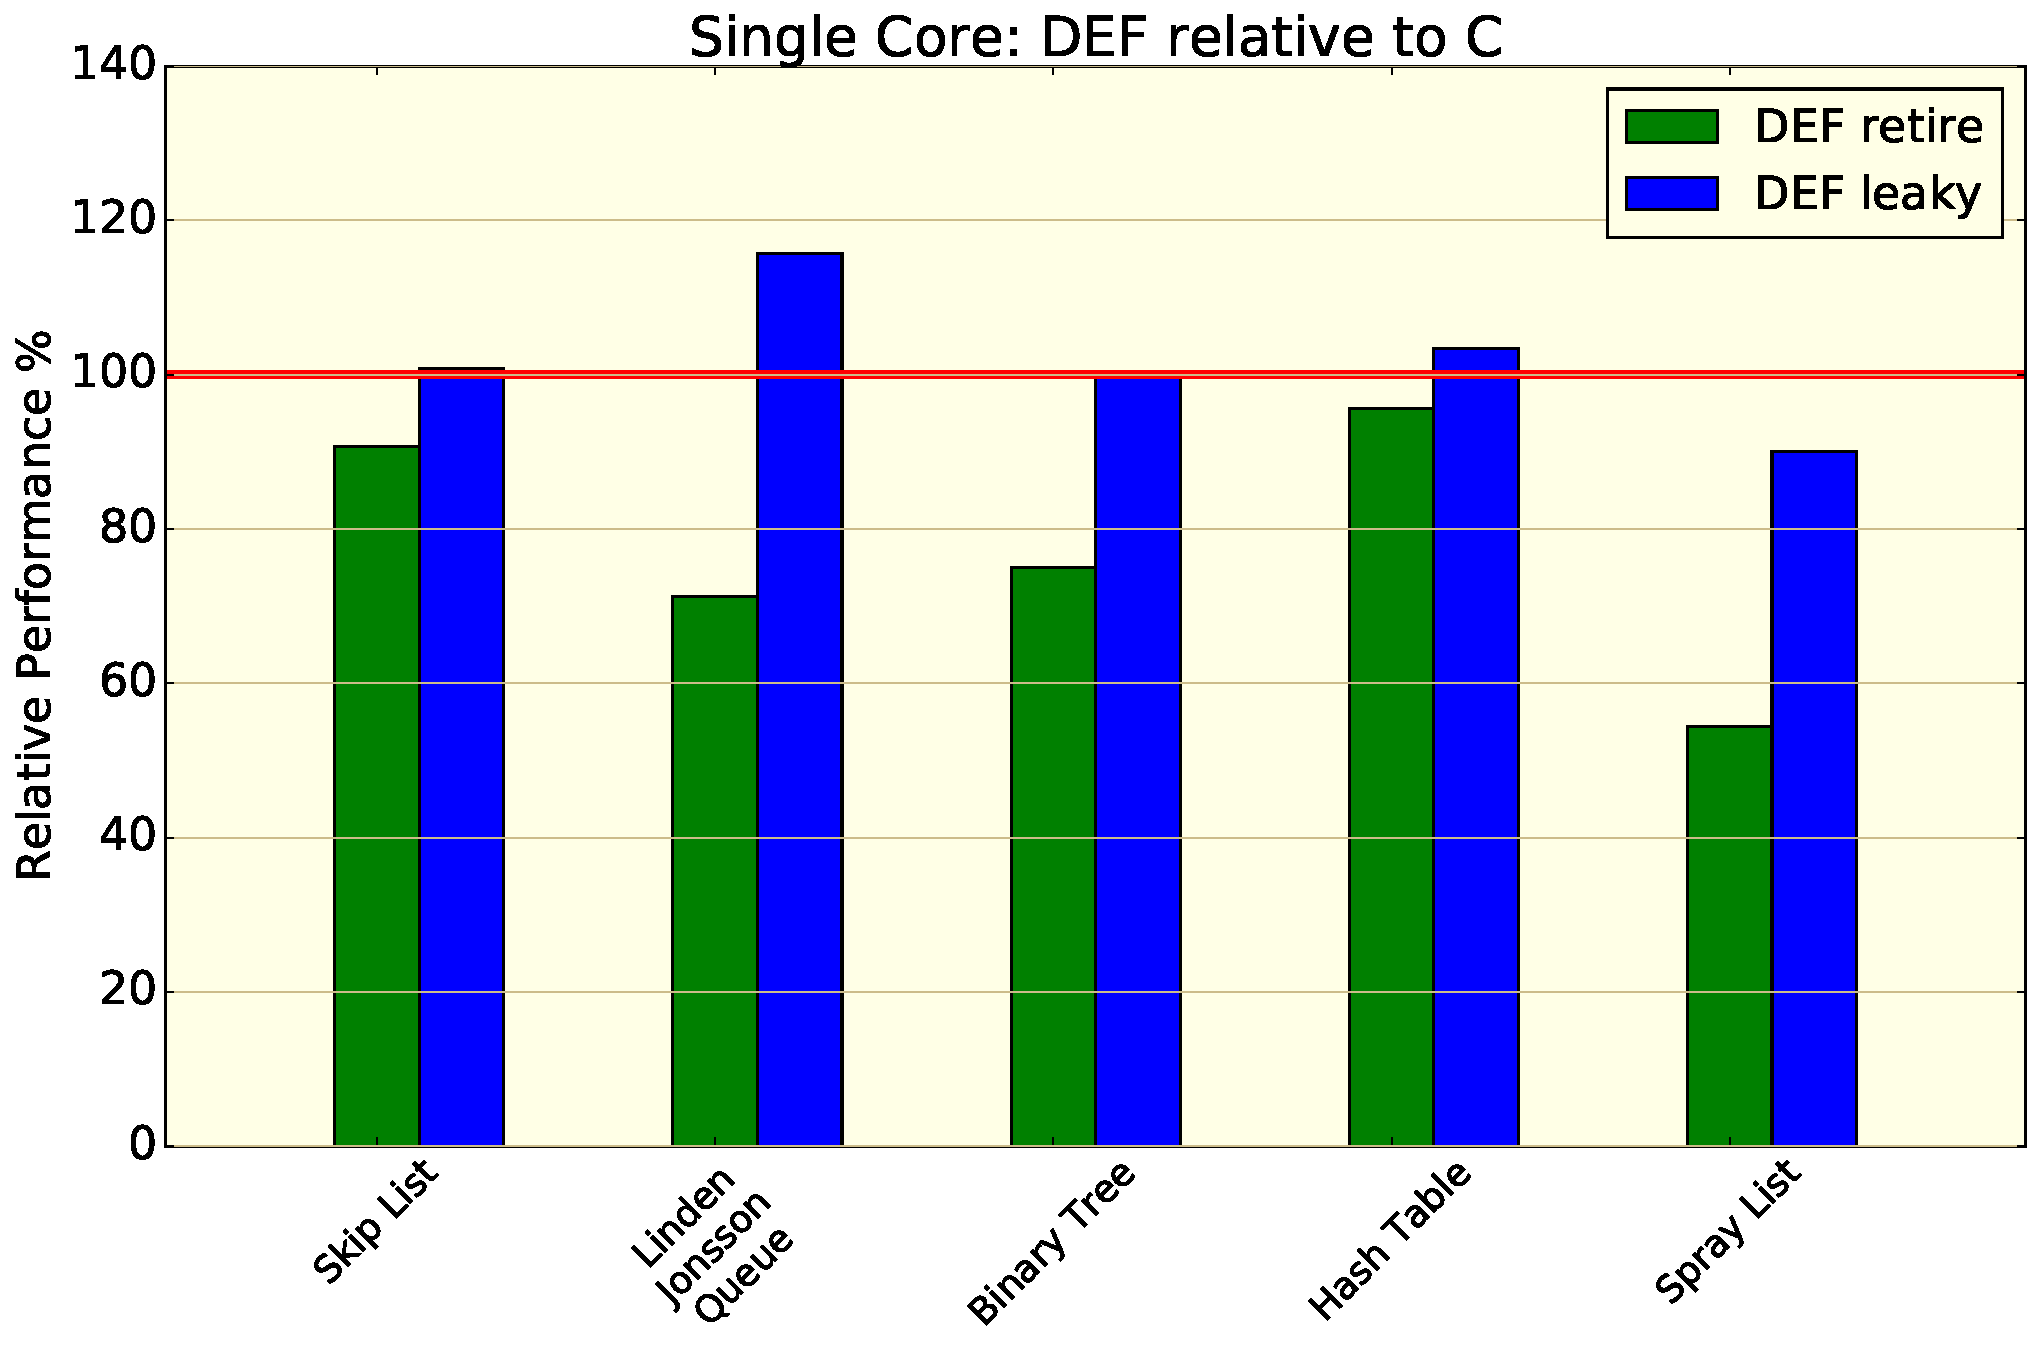
\includegraphics[scale=0.4]{gfx/RelativePerf.pdf}
\caption{Relative performance of C to DEF}
\label{fig:relativeperf}
\end{figure}

\begin{figure}
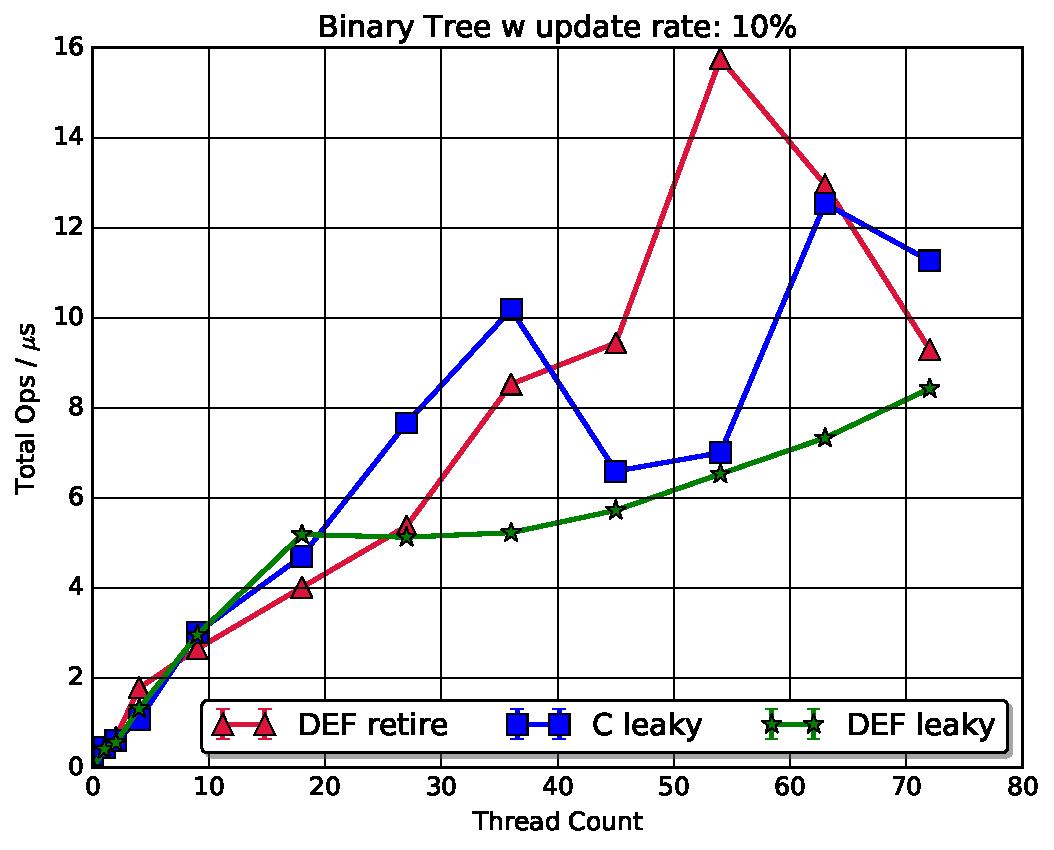
\includegraphics[scale=.4]{gfx/BinaryTreeLight.pdf}
\caption{Lock-Free Binary Tree}
\label{fig:bintreelight}
\end{figure}

\begin{figure}
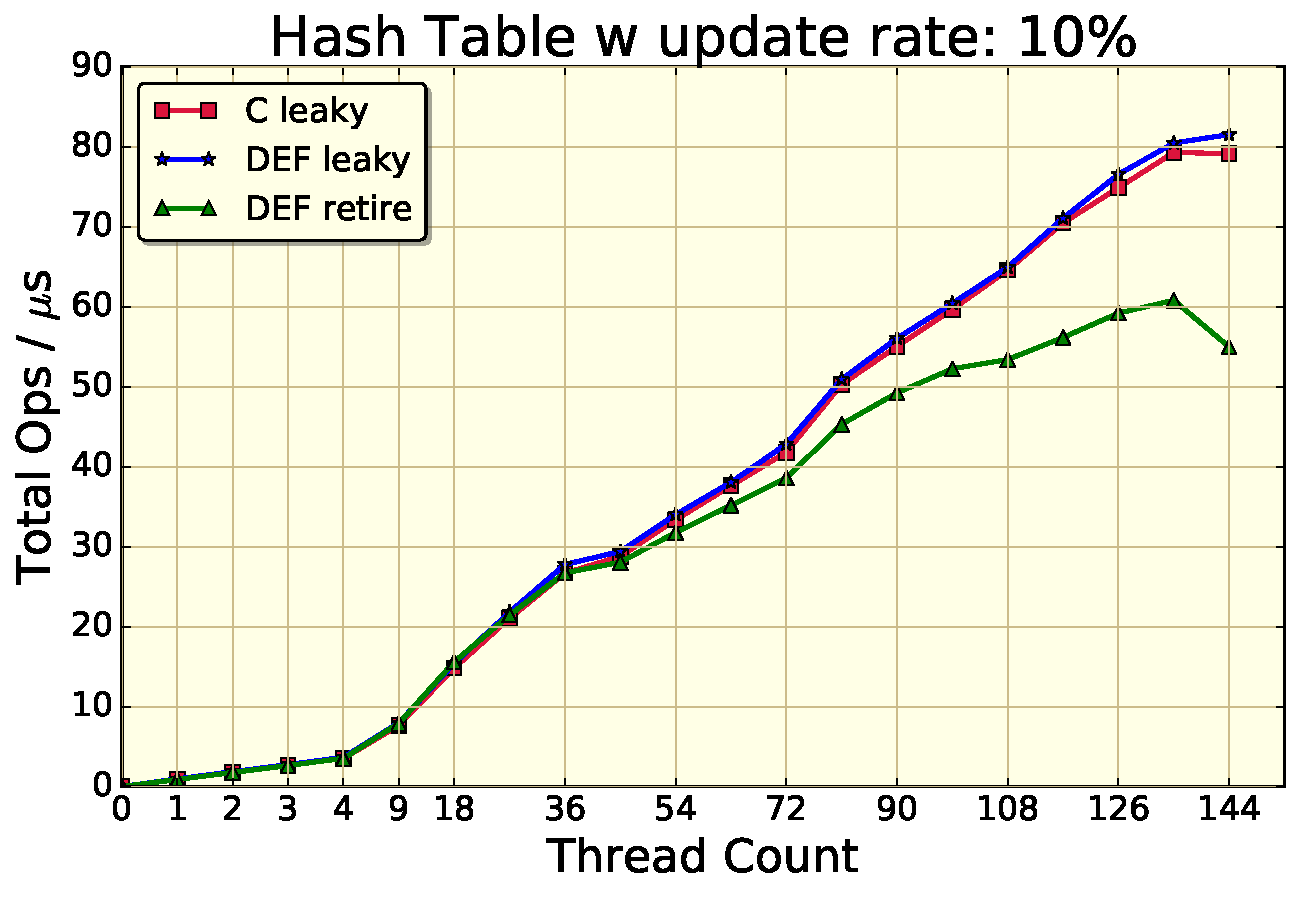
\includegraphics[scale=.4]{gfx/HashTableLight.pdf}
\caption{Lock-Free Hash Table}
\end{figure}

\begin{figure}
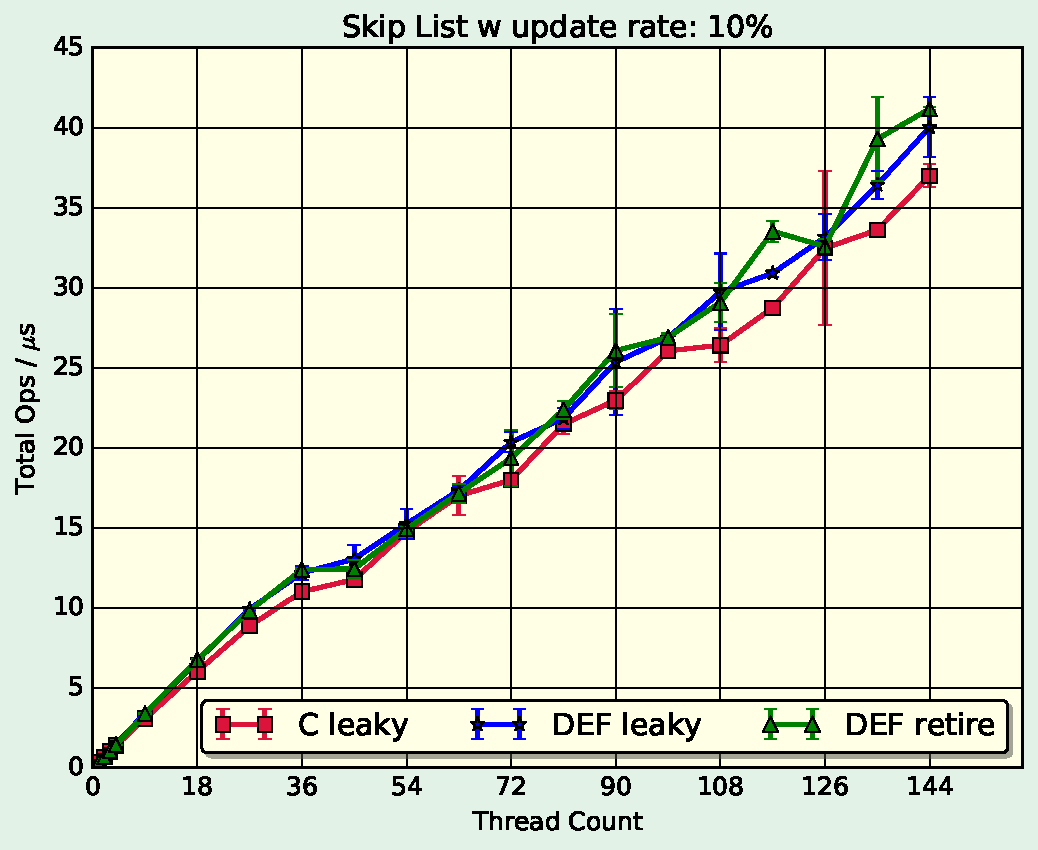
\includegraphics[scale=.4]{gfx/SkipListLight.pdf}
\caption{Lock-Free Skip List}
\end{figure}

\begin{figure}
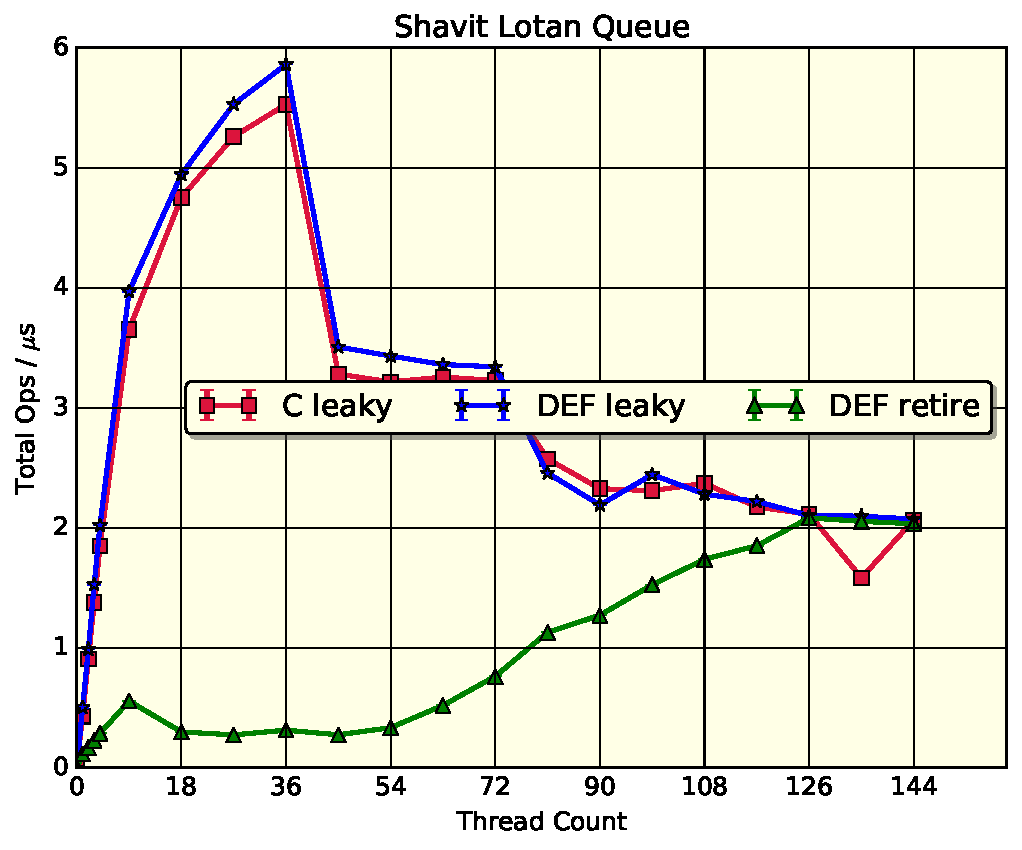
\includegraphics[scale=.4]{gfx/ShavitLotanQueue.pdf}
\caption{Lock-Free Priority Queue}
\end{figure}

\begin{figure}
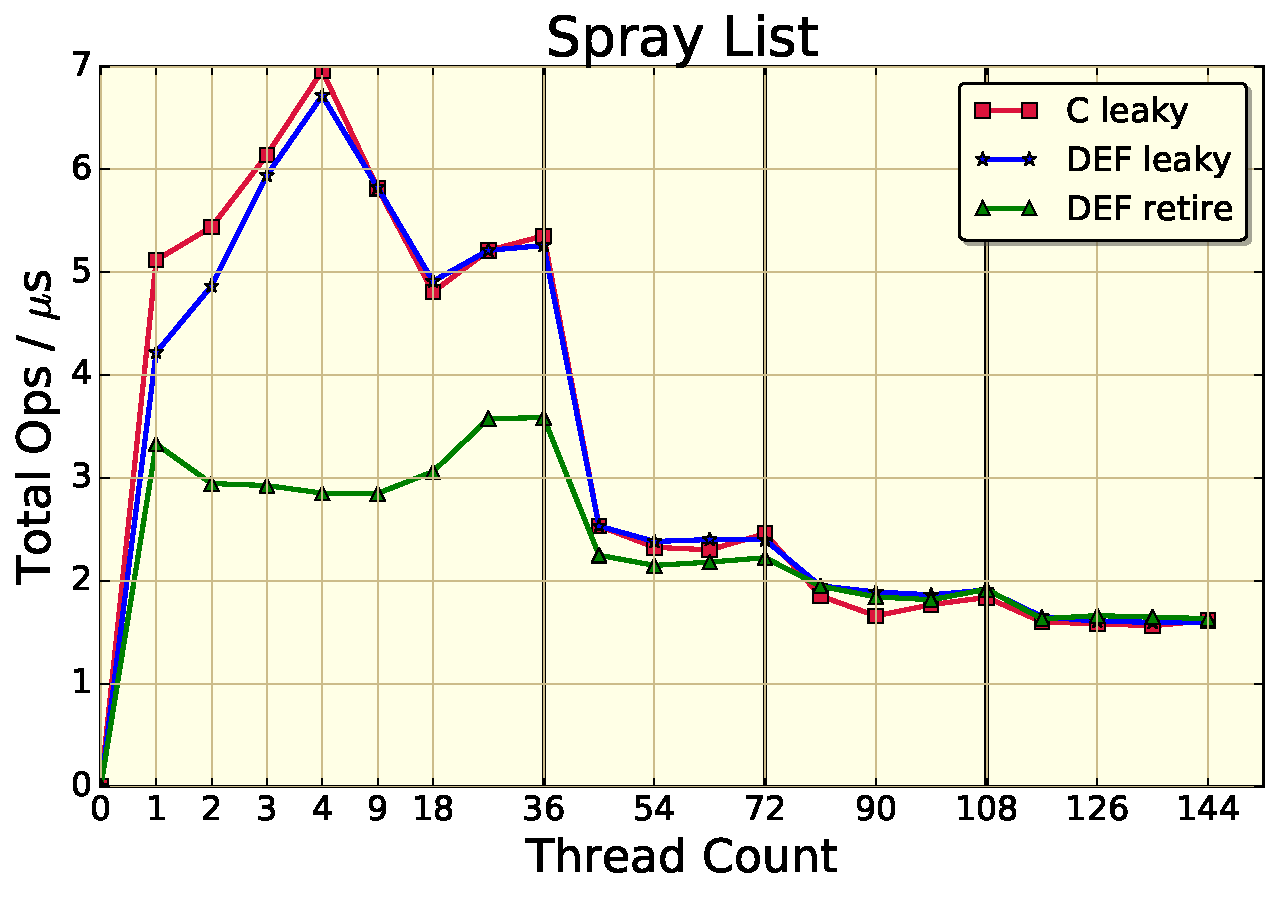
\includegraphics[scale=.4]{gfx/SprayList.pdf}
\caption{Spray List Priority Queue}
\end{figure}

\subsection{Experimental Results}
